\section{Problemi di Search}
L'insieme dei problemi di Search è un insieme di problemi legati all'inferenza (piuttosto che al Machine Learning). 
Tali problemi vengono formulati e risolti da un agente per trovare il percorso che li porterà ad uno stato obiettivo;
per fare ciò, considereremo un ambiente che è:
\begin{itemize}
    \item \textbf{Statico} dal momento che assumiamo che durante la ricerca il mondo non cambi (altrimenti la ricerca sarà inutile)
    \item \textbf{A Singolo Agente} per semplificare la situazione
    \item \textbf{Completamente Osservabile} per poter conoscere lo stato iniziale dell'agente
    \item \textbf{Discreto} in modo da poter descrivere i passi risolutivi in maniera discreta
    \item \textbf{Deterministico} perchè ad ogni azione devo essere sicuro del suo effetto per la computazione dello stato successivo
\end{itemize}
\subsection{Formulazione del Problema}
Per la descrizione dei problemi di Search useremo queste convenzioni:
\begin{itemize}
    \item $S = \{ s_1, s_2, \dots\}$ è detto \textit{Insieme degli stati} (deve essere finito)
    \item $s_i \in S$ è detto \textit{stato iniziale}
    \item $s_G \in S$ è detto \textit{stato di Goal} (può essere più di uno)
    \item $A(s_i) = \{ a,b,c,\dots\}$è \textit{l'insieme delle azioni possibili allo stato i}
    \item $f(s_i,a)$ con $s_i \in S$ e $a \in A(s_i)$ è detto \textit{modello di Transizione} o \textit{Funzione Successore}; corrisponde allo lo stato successivo
    \item $c(s_i,a,f(s_i,a))$ è detto \textit{costo Additivo}. Una cosa da tenere a mente per il costo additivo
    è che i vari costi devono poter essere tutti sommabili (non possono essere grandezze diverse)
\end{itemize}

Un'altra formulazione interessante del problema usa il \textit{Grafo degli Stati}, dove gli archi sono le azioni e i nodi sono gli
stati.

\subsection{Classificazione dei problemi}
In base a cosa cercare, i problemi di Search possono essere di 3 tipi:
\begin{itemize}
    \item \textbf{Fattibilità} \label{def:fattibilità} \\ 
    I problemi di Fattibilità hanno come obiettivo di rispondere la domanda: \textit{Esiste un percorso che mi porta da $s_i$ ad un $s_G$?}.
    In questi problemi bisogna quindi esplorare un qualunque percorso che mi porti all'uscita del labirinto, senza sapere necessariamente la sequenza di azioni o quella più efficiente/interessante.
    \item \textbf{Approssimazione}\\
    I problemi di Approssimazione, invece, ricercano una soluzione che soddisfi alcune garanzie (es: "il percorso trovato dev'essere al massimo il 30\% peggiore dell'ottimo").
    Chiaramente questi tipi di algoritmi sono difficili da progettare dal momento che dimostrare tali garanzie è davvero arduo.
    \item \textbf{Ottimizzazione}\\
    Sono problemi che richiedono il percorso più bello/efficiente/interessante rispetto a tutti gli altri (e di dimostrarlo) che mi porti allo stato obiettivo.
\end{itemize}
In generale dobbiamo dire che, negli ultimi 2 casi, il risultato del problema di Search è un \href{https://it.wikipedia.org/wiki/Albero_(informatica)}{albero} la cui radice è lo stato iniziale e in cui un ramo porta allo stato obiettivo.

\subsection{Approccio Esaustivo/Esplicito}
Un primo approccio che potremmo formulare, per risolvere tali problemi, è quello di
precalcolare tutti i possibili percorsi e selezionare quello più efficiente. Chiaramente questo approccio è INUTILIZZABILE
in problemi di dimensione reale (ma nemmeno troppo grandi): tutti i possibili passi per la risoluzione del Cubo di Rubik, per esempio, sono
circa $4,33 * 10^{43}$ permutazioni, cosa che non è possibile contenere tutta in memoria.

\subsection{Approccio Implicito}
In questo caso, invece, piuttosto che enumerare tutti i possibili percorsi, si esplorano solo quelli più "interessanti" a partire dallo stato iniziale. Dunque,
piuttosto che tenere in memoria tutti i possibili percorsi, tengo solo quelli che effettivamente ho esplorato ed eventualmente scarto quelli non ottimi.

\subsection{Caratteristiche di un Algoritmo}
D'ora in poi, gli algoritmi di Search che mostreremo nel corso verranno valutati in base ai seguenti parametri:
\begin{itemize}
    \item \textbf{Correttezza}: questa proprietà afferma che, se l'algoritmo restituisce un risultato, questo dev'essere conforme alle specifiche 
    (cioè, se si richiede, per esempio, di trovare il percorso migliore, il risultato dell'algoritmo DEVE RESTITUIRE IL PERCORSO MIGLIORE)
    \item \textbf{Completezza}: se esiste una soluzione al problema, l'algoritmo la troverà sempre. In altri termini, l'algoritmo deve sempre terminare con una risposta in un tempo finito. 
    Nel caso in cui i passi del problema sono infiniti (ovviamente contabili), la completezza viene detta \textbf{Sistematicità} e va dimostrata.
    \item \textbf{Complessità Spaziale}: l'uso (nel caso peggiore) della risorsa spaziale (memoria disponibile) per la risoluzione del problema in funzione della dimensione dell'input
    \item \textbf{Complessità Temporale}: l'uso (nel caso peggiore) della risorsa temporale (passi da eseguire) per la risoluzione del problema in funzione della dimensione dell'input
\end{itemize}


\subsection{Problema di Riferimento}
Per presentare i seguenti algoritmi, ci riferiremo sempre a questo grafo, in cui gli archi sono bidirezionali 
(ossia, per ogni $X,Y$ stati del problema $c(X,a,Y) = c(Y,b,X)$ con $a$ l'arco di transizione da $X$ a $Y$ e $b$ l'arco di transizione da $Y$ ad $X$) \\
\begin{center}
    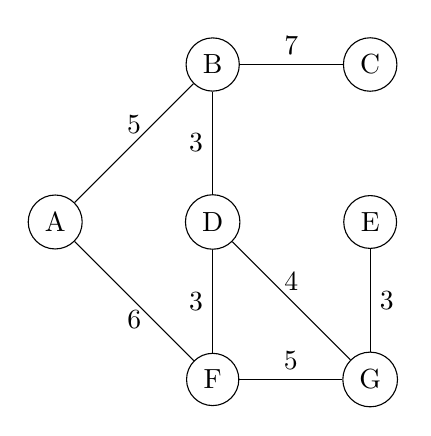
\begin{tikzpicture}
        % Nodi
        \node[circle, draw] (A) at (0,0) {A};
        \node[circle, draw] (B) at (2,2) {B};
        \node[circle, draw] (D) at (2,0) {D};
        \node[circle, draw] (F) at (2,-2) {F};
        \node[circle, draw] (C) at (4,2) {C};
        \node[circle, draw] (G) at (4,-2) {G};
        \node[circle, draw] (E) at (4,0) {E};
    
        % Archi
        \draw[-] (A) -- (B) node[midway, above] {5}; % Arco da A a B
        \draw[-] (A) -- (F) node[midway, below] {6}; % Arco da B a D
        \draw[-] (B) -- (D) node[midway, left] {3}; % Arco da D a C
        \draw[-] (D) -- (F) node[midway, left] {3}; % Arco da C a A
        \draw[-] (B) -- (C) node[midway, above] {7}; % Arco da C a A
        \draw[-] (D) -- (G) node[midway, above] {4}; % Arco da C a A
        \draw[-] (F) -- (G) node[midway, above] {5}; % Arco da C a A
        \draw[-] (G) -- (E) node[midway, right] {3}; % Arco da C a A
    
    \end{tikzpicture}
\end{center}

I vari algoritmi che presenteremo differiscono per come rispondono alla domanda: "\textit{Dato che ho ispezionato il nodo, proseguo o vado indietro?}"


\subsection{Ricerca Non Informata}
\subsubsection{Depth-First-Search} \label{alg: dfs}
Un algoritmo classico di ricerca su grafo è la ricerca in profondità. In questa versione, la DFS è dotata di \textit{Backtracking}. Possiamo 
dire in generale che l'approccio di questo algoritmo è aggressiva, poichè ricerca subito in profondità la soluzione (potrebbe metterci molto o potrebbe metterci poco), ossia non c'è garanzia.
Inoltre possiamo osservare che gli alberi generati dalla DFS sono stretti e lunghi.\\
\smallskip
\textbf{Funzionamento:}
\begin{enumerate}
    \item Si parte dal nodo iniziale A (che sarà poi radice dell'albero finale)
    \item Se il nodo da esplorare ha dei figli, si aggiungono all'albero i vari figli; in caso ve ne sia più di uno,
    un \textit{Tie-Breaker} spesso usato è basato sull'ordine lessicografico (quindi, per esempio, se esploriamo A, il primo figlio da esplorare sarà B)
    \item Si torna indietro se: il nodo è foglia, oppure se il nodo è già stato visitato
\end{enumerate}

\textbf{Analisi}:
\begin{itemize}
    \item \textbf{Correttezza}: La dfs restituisce sempre un albero (grazie all'uso del Backtracking e all'eliminazione dei loop)
    \item \textbf{Completezza}: La dfs restituisce sempre un albero in cui un ramo contiene lo stato obiettivo (se esiste il percorso)
    \item \textbf{Complessità Temporale}: Dato b il \textit{Branching Factor} e d la \textit{profondità massima}, la complessità di tale algoritmo è esponenziale, ossia $O(b^d)$
    \item \textbf{Complessità Spaziale}: La memoria usata è quella necessaria per generare l'albero; in questo caso la complessità è $O(d)$ ossia la profondità massima del percorso dallo start al goal.

\end{itemize}

\subsubsection{Breath-First-Search}
Un altro algoritmo classico di ricerca su grafo è la ricerca in ampiezza. Anche la BFS è dotata di \textit{Backtracking}. Possiamo 
dire in generale che l'approccio di questo algoritmo è conservativa, poichè ricerca sempre allo stesso livello, garantendo di visitare tutti i nodi.
Possiamo inoltre dire che gli alberi generati dalla BFS sono larghi e corti.\\
\smallskip
\textbf{Funzionamento:}
\begin{enumerate}
    \item Si parte dal nodo iniziale A (che sarà poi radice dell'albero finale)
    \item Se il nodo padre ha dei figli da esplorare, vengono tutti aggiunti all'albero; Si prosegue poi ai figli del primo nodo figlio e così via.
    Il \textit{Tie-Breaker} che possiamo usare è ancora quello basato sull'ordine lessicografico.
    \item Si torna indietro se: il nodo è foglia, oppure se il nodo è già stato visitato
\end{enumerate}

\textbf{Analisi}:
\begin{itemize}
    \item \textbf{Correttezza}: Per lo stesso motivo della DFS
    \item \textbf{Completezza}: Per lo stesso motivo della DFS
    \item \textbf{Complessità Temporale}: Dato b il \textit{Branching Factor} e q la \textit{profondità minima}, la complessità di tale algoritmo è esponenziale, ossia $O(b^q)$ (quindi sempre minore, nel caso peggiore, della DFS)
    \item \textbf{Complessità Spaziale}: In questo caso, dato che non viene allocata altra memoria se non il grafo stesso, la complessità spaziale sarà $O(n)$ con n il numero di nodi. 
\end{itemize}
\subsubsection{DFS/BFS Ottimizzati}
Gli ultimi 2 algoritmi possono essere ottimizzati introducendo nuove strutture dati, usate per evitare di rivisitare 
i nodi e quindi per generare alberi più piccoli:

\paragraph{EQL (Enqueued List).}
La EQL, anche detta \textit{lista di accodamento}, è una lista che tiene traccia di tutti i nodi già visitati; è detta
di accodamento perchè ad ogni nuova visita, il nodo visitato viene aggiunto alla fine; quando si deve vistare un nodo
si verifica che questo non sia già nella lista; se lo è, tutto il sottoalbero relativo non verrà esplorato. Questa 
operazione è detta \textbf{Potatura} o \textbf{Pruning}

\paragraph{Frontiera.}
Definiamo frontiera l'insieme dei nodi foglia non ancora espansi dell'albero; è detta così dal momento che, per la
\textbf{Separation Property}, separa la parte dell'albero esplorata da quella ancora non esplorata.\\
Implementazioni della Frontiera:
\begin{itemize}
    \item \textbf{Caso BFS}: la frontiera viene implementata come \textbf{Queue} (una coda FIFO)
    \item \textbf{Caso DFS}: la frontiera viene implementata come \textbf{Stack} (una coda LIFO)
\end{itemize}

\textbf{Analisi}:
\begin{itemize}
    \item \textbf{Correttezza}: L'uso delle EQL pota solo i sottoalberi già esplorati, per cui la correttezza non viene compromessa
    \item \textbf{Completezza}: L'algoritmo è ancora completo per il motivo precedente
    \item \textbf{Complessità Temporale/Spaziale}: anche se abbiamo introdotto queste strutture dati per ottimizzare le operazioni,
          in realtà la complessità nel caso peggiore non cambia. Grazie a queste ottimizzazioni, tuttavia, è possibile usare in un tempo ragionevole
          i 2 algoritmi
\end{itemize}
